
\section{Discussion}

In this article, we discussed the SUPERTREX model presented by
\textcite{pyle2019}. We compared the results presented in the paper,
both with the results obtained using the original scripts, and with our modular and user-friendly Python adaptation. Furthermore, we were able to improve the robustness and scalability of the model with two minor alterations.

The Python adaptation strives to be a close adaptation of the original scripts in MATLAB and differs mainly in the method of initialisation of the reservoir connectivity matrix. This is due to the usage of the function {\tt sprandn} in the original scripts, whose internal implementation is not freely available. Figure~\ref{Fig:Comparison_sprandn} shows that, on importing initialisation matrix from MATLAB, the exact same results can be obtained in the Python adaptation, as well. Most of the details for the implementation of the models are also described in the paper. Only two necessary details were missing, both concerning the update of the readout weights of the exploratory pathway in the RMHL and SUPERTREX models: One, the inclusion of a crucial learning rate of 0.0005, for Tasks 1-3, and two, an additional compensatory factor of 0.5, for Task 3. There is another discrepancy in the function $psi(x)$ for Task 3. The scripts provided by the authors use a factor of 0.005, whereas the article mentions this factor to be 0.025.

The three algorithms (FORCE, RMHL and SUPERTREX) have been tested on three tasks, presented in \textcite{pyle2019}. For Task 1 and 2, we verify that the three algorithms function as presented in the paper, and validate that our Python re-implemen\-tation produces comparable results. For Task 3, the SUPERTREX model's behaviour is also reproducible, although the performance is dependent on the seed used for the random number generator. Furthermore, we observed that this implementation is quite sensitive to changes in task parameters, such as the number of arms. This was due to the uninhibited increase in the readout weights. We propose the inclusion of a compensation factor for the number of arm segments, which inhibits the growth of the readout weights, and allows the simulation to proceed in a meaningful manner. This considerably improves the robustness and the scalability of the original model.\\

We conclude that the results presented in the paper are  reproducible for two tasks, using the original MATLAB scripts provided by the authors, and also, replicable in Python for all tasks with comparable performance.



\begin{figure}[h]


    \centering
    
    % \hspace{2em}
    \textbf{MATLAB}\hspace{14em}
    \textbf{Python}
    
    \hspace{-2em}
    
\includegraphics[trim=3cm 4cm 3cm 4cm, clip=true, height=.25\linewidth]{Figures/Fig_T7/MATLAB/RMHL_T1_Trajectory.eps}
    \hspace{4em}
    
\includegraphics[trim=6.5cm 4.5cm 6cm 4.5cm, clip=true,  height=.25\linewidth]{Figures/Fig_T7/Python/RMHL_T1_Jmat_Trajectory.eps} \\
    
    
    
    
        \textbf{\rotatebox[origin=c]{90}{x(t)}}\begin{subfigure}{\textwidth}
        \centering
        
        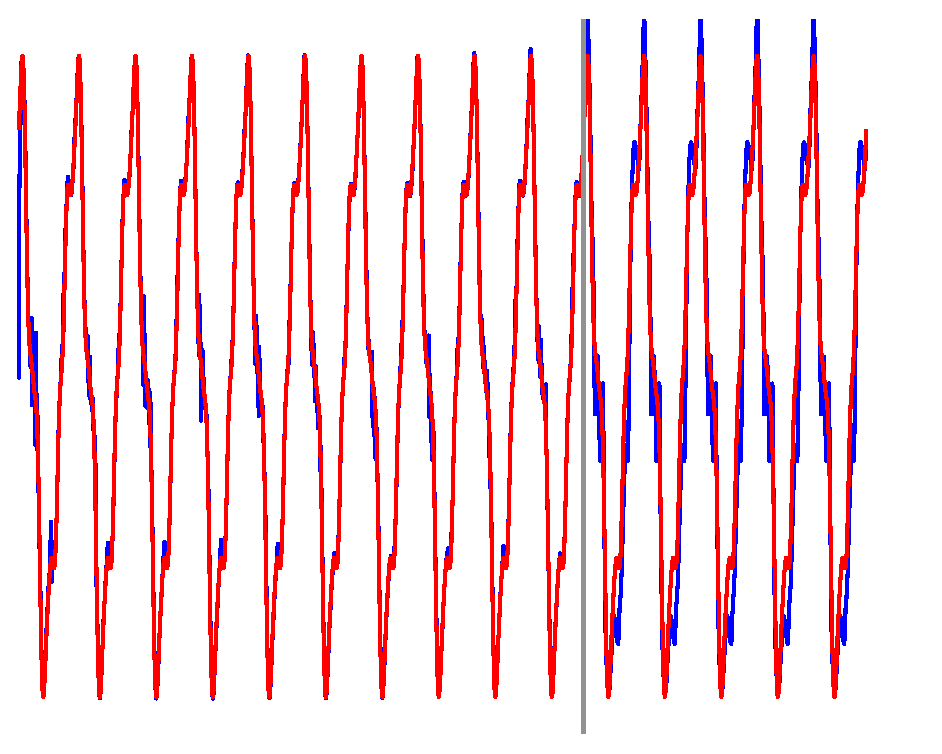
\includegraphics[trim=0cm 0cm 0cm 0cm,clip=true,height=0.1\linewidth,width=.45\linewidth]{Figures/Fig_T7/MATLAB/RMHL_T1_CoordinateX.eps}
        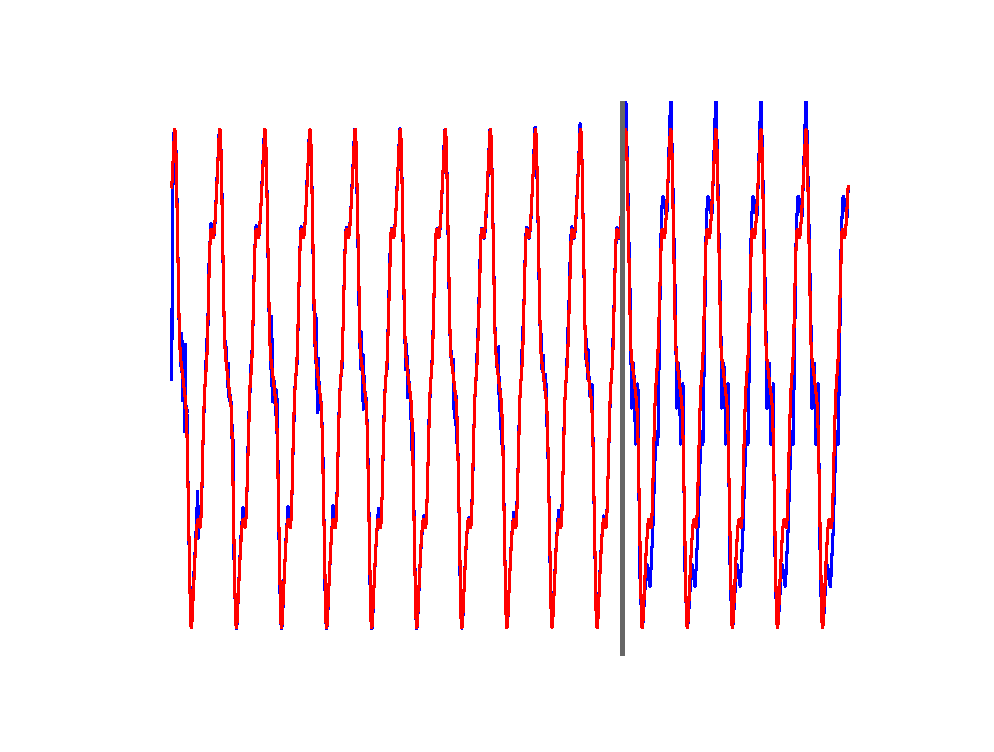
\includegraphics[trim=2cm 1cm 2cm 1cm,clip=true,height=0.1\linewidth,width=.45\linewidth]{Figures/Fig_T7/Python/RMHL_T1_Jmat_CoordinateX.eps}\\
    
    \end{subfigure}
    
    
        \textbf{\rotatebox[origin=c]{90}{y(t)}}\begin{subfigure}{\textwidth}
        \centering
        
        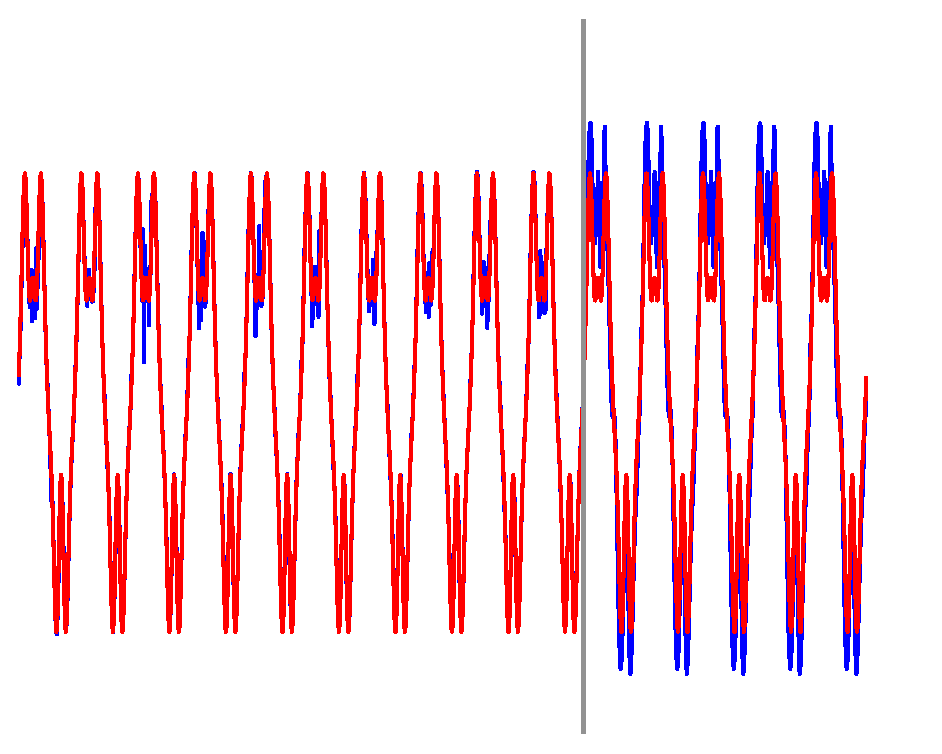
\includegraphics[trim=0cm 0cm 0cm 0cm,clip=true,height=0.1\linewidth,width=.45\linewidth]{Figures/Fig_T7/MATLAB/RMHL_T1_CoordinateY.eps}
        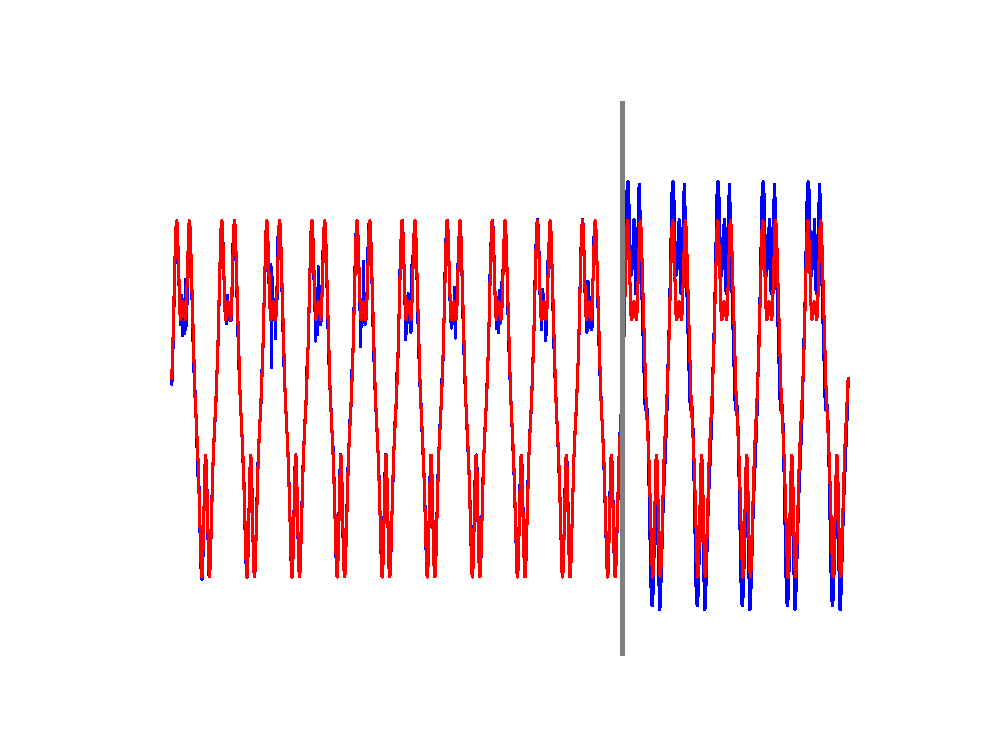
\includegraphics[trim=2cm 1cm 2cm 1cm,clip=true,height=0.1\linewidth,width=.45\linewidth]{Figures/Fig_T7/Python/RMHL_T1_Jmat_CoordinateY.eps}   
    
    \end{subfigure}
    
    
    \vspace{4em}
    
    \textbf{\rotatebox{90}{$||W||$}}\begin{subfigure}{\textwidth}
        \centering
        
        \hspace{.5em}
        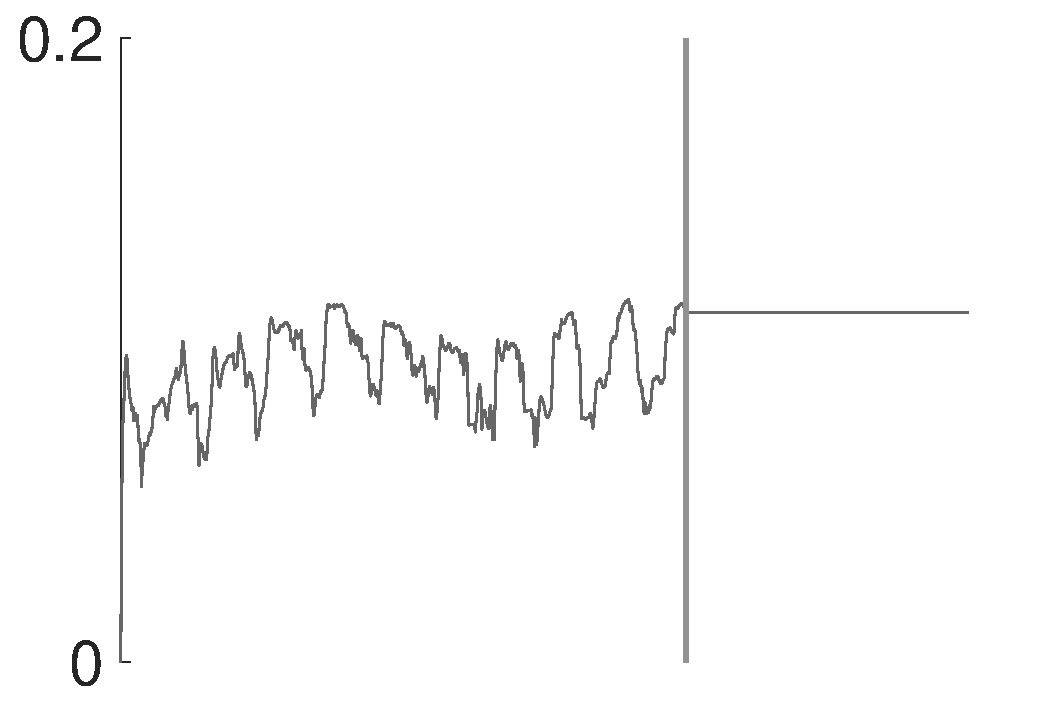
\includegraphics[trim=0cm 0cm 0cm 0cm,clip=true,height=0.15\linewidth,width=.45\linewidth]{Figures/Fig_T7/MATLAB/RMHL_T1_W_norm.eps}
        \hspace{0em}
        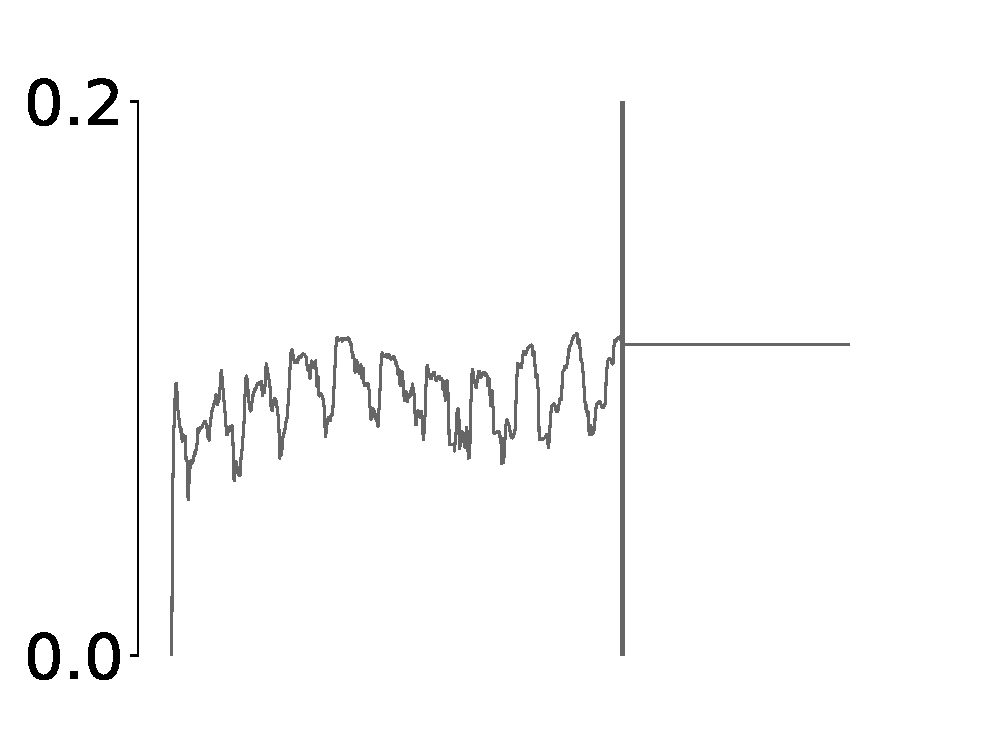
\includegraphics[trim=0cm 0.5cm 2cm 0.5cm,clip=true,height=0.15\linewidth,width=.45\linewidth]{Figures/Fig_T7/Python/RMHL_T1_Jmat_W_norm.eps}
    
    \end{subfigure}
    
    
    \vspace{2em}
    
    \textbf{\rotatebox{90}{MSE}}\begin{subfigure}{\textwidth}
        \centering
        
        \hspace{.5em}
        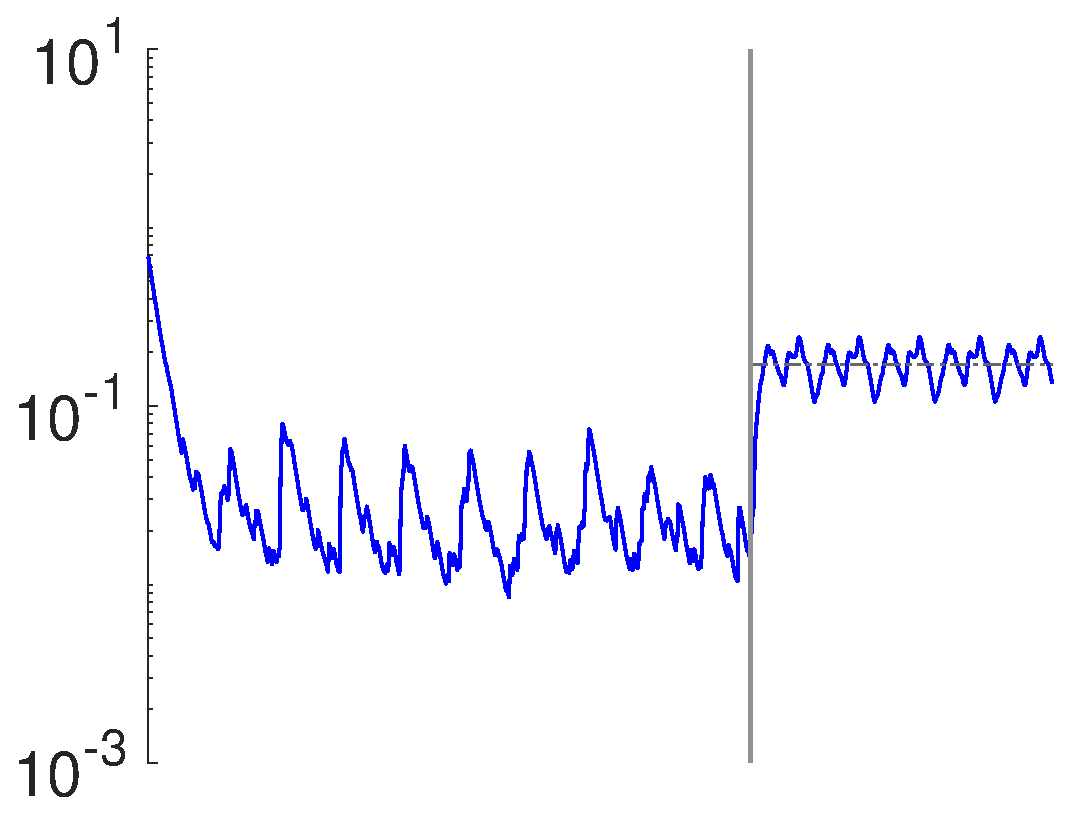
\includegraphics[trim=0cm 0cm 0cm 0cm,clip=true,height=0.15\linewidth,width=.45\linewidth]{Figures/Fig_T7/MATLAB/RHML_T1_Jmat_MSE.eps}
        \hspace{1em}
        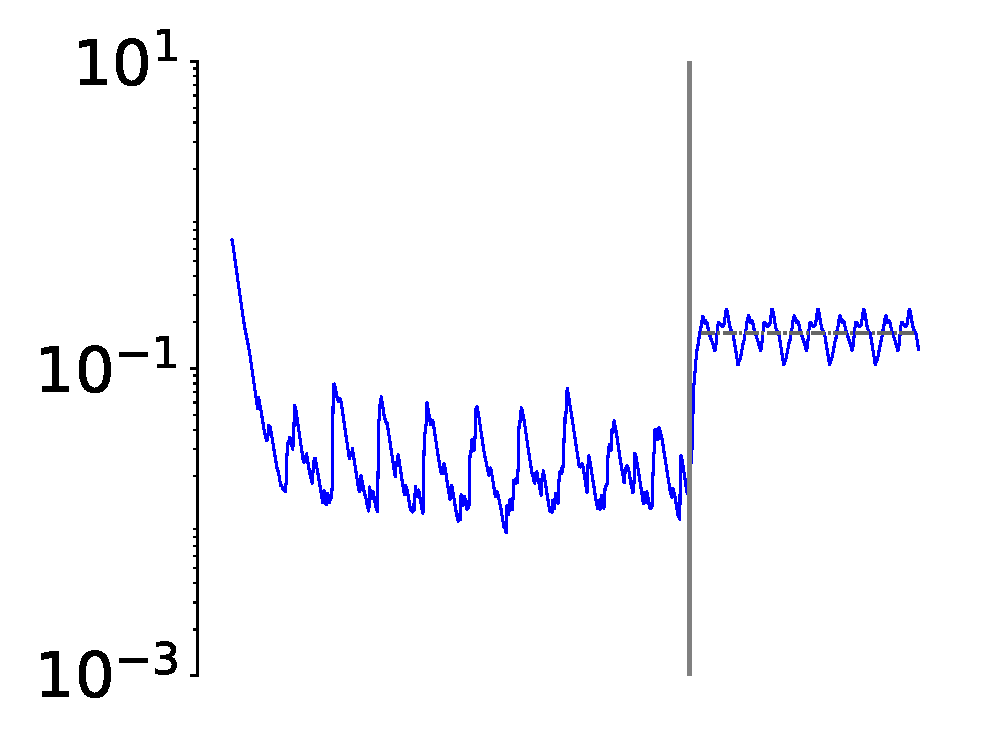
\includegraphics[trim=0cm 0cm 0cm 0cm,clip=true,clip=true,height=0.15\linewidth,width=.45\linewidth]{Figures/Fig_T7/Python/RMHL_T1_Jmat_MSE.eps}
    
    \end{subfigure}
        
            

        
    
        
        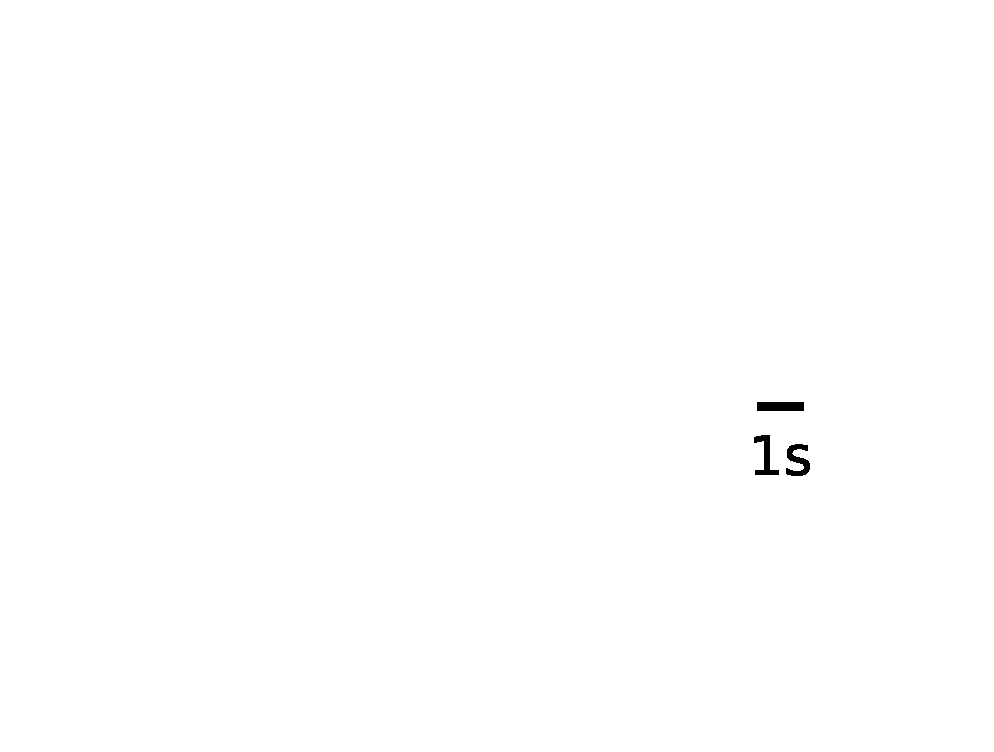
\includegraphics[trim=2cm 6cm 2cm 6cm, clip=true,height=0.05\linewidth,width=.4\linewidth]{Figures/Fig_T1/Python/ST_T1_Scale.eps}
        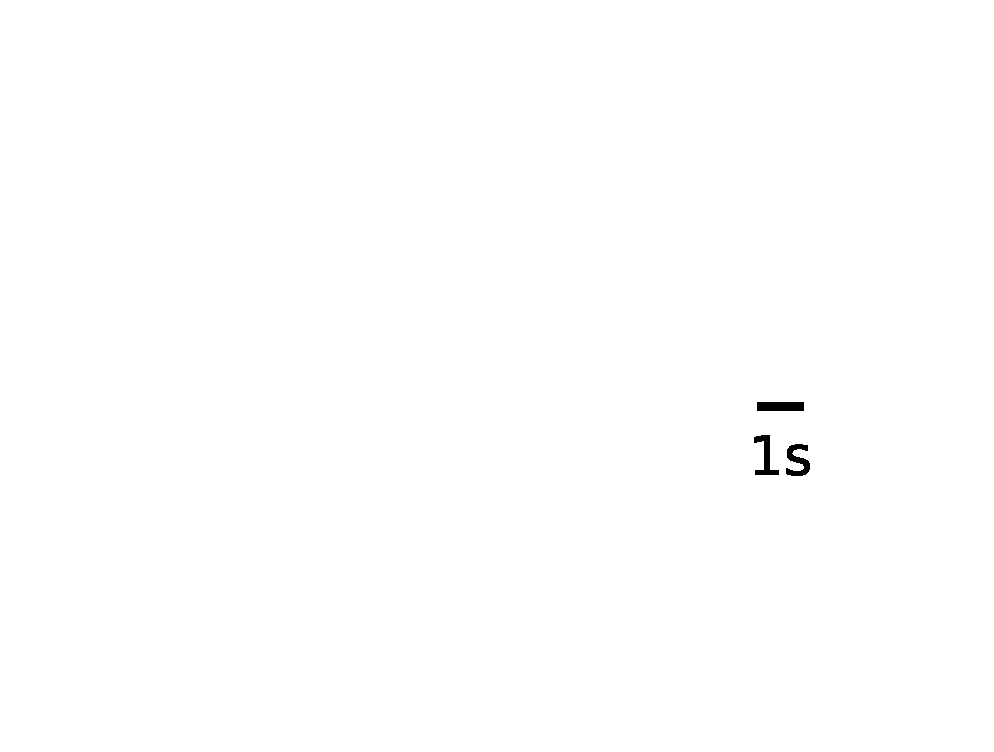
\includegraphics[trim=2cm 4cm 2cm 6cm, clip=true,height=0.05\linewidth,width=.45\linewidth]{Figures/Fig_T1/Python/ST_T1_Scale.eps}


\caption{Similarity between the original scripts and the Python adaptation. The performance of the original scripts (left column) and the Python adaptation (right column) is tested for the RMHL learning algorithm on a Task 1. The reservoir connectivity matrix for the Python simulation was initialised using the MATLAB equivalent. Using this initialisation, the progression of the Python simulation is identical to that of the MATLAB simulation. The top panel shows the target trajectory (red) with the trajectory generated by the model (blue) throughout the test phase. The next two rows show the time-series (blue) generated by the model (x and y coordinates, in this case). The third row shows the progression of the norm of the weight matrix. The bottom row shows the distance from target metric (blue) over the simulation, using the log scale for the y axis. The horizontal grey line, in the test phase, indicates the deviation metric. The grey vertical line marks the separation of the training and testing phase.}
\label{Fig:Comparison_sprandn}

\end{figure}